\chapter{Project 2: High-resolution segmentation (Satellite\_based\_tile\_segmentation)}

\section{Why this project matters for a pathology company}
A 6000$\times$6000 aerial tile and a 100k$\times$200k WSI pose the same engineering questions: the network sees
256$\times$256 patches, so we need patch extraction, class-imbalance handling (cars $\approx$1\% of pixels $\leftrightarrow$
tumour cells), multi-scale context (buildings vs cars $\leftrightarrow$ glands vs nuclei), stitching without seams, and
test-time augmentation. \textbf{Segmentation} = assigning a class to every pixel.
\begin{figure}[H]\centering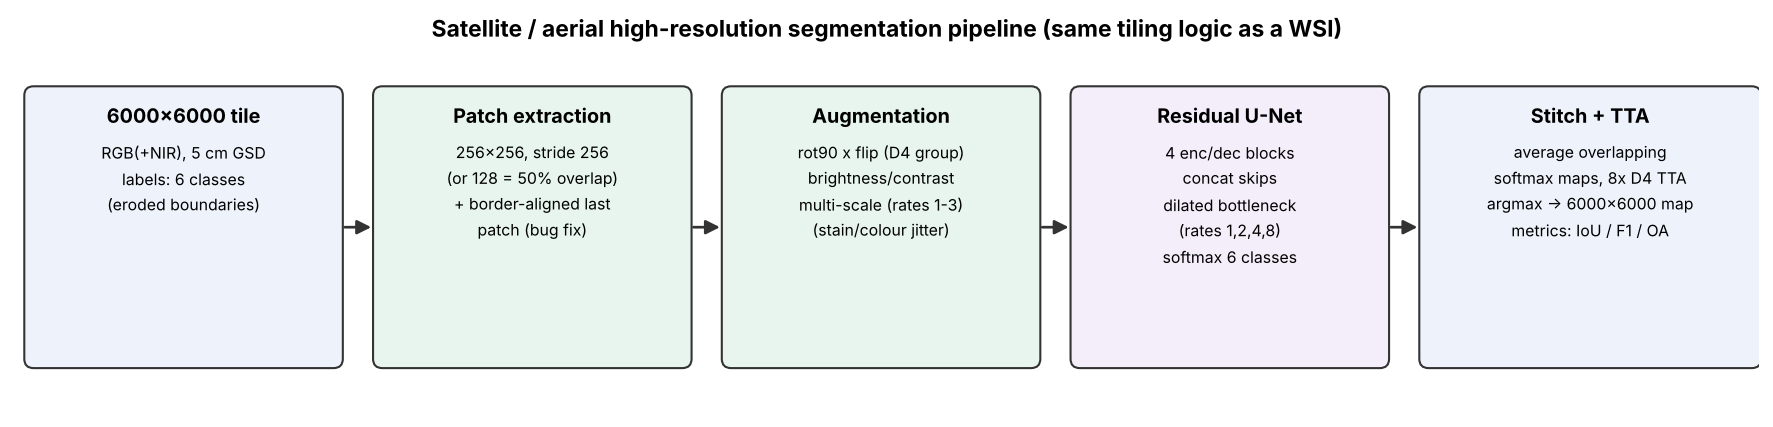
\includegraphics[width=\linewidth]{pipeline_satellite.png}\caption{Satellite segmentation pipeline.}\end{figure}

\section{Architecture (as implemented in the repo)}
\begin{itemize}
\item Input 256$\times$256$\times$3, 4 encoder blocks (filters 32$\to$256 with \texttt{filters=32}), each two
3$\times$3 conv + BN + ReLU, ``residual'' = concatenation of block input and output, 2$\times$2 max-pool.
\item Bottleneck: dilated convolutions with rates 1, 2, 4, 8 (serial or parallel), concatenated -- ASPP-like
multi-scale context.
\item Decoder: 2$\times$2 transposed conv, concatenate skip, two convs (+ concat ``residual''); 1$\times$1 conv + softmax
over 6 classes (impervious, building, low vegetation, tree, car, clutter).
\item Training aids in repo: LR range test (Smith 2015), one-cycle policy (Smith 2018), Jaccard and focal losses,
multi-scale patch extraction (\texttt{tf.image.extract\_patches} with rates 1--3), flips/rotations/colour jitter.
\item Inference: patches $\to$ predict $\to$ average overlapping softmax maps $\to$ argmax; 8$\times$ $D_4$ TTA.
\end{itemize}
Model size: 16.5\,M parameters with \texttt{filters=32}, 4.1\,M with \texttt{filters=16} (we measured 6.4\,s vs 1.9\,s per
batch of 8 on CPU).

\section{Bugs and over-claims found}
\begin{enumerate}
\item \textbf{Border pixels never predicted}: \texttt{range(0, h-p+1, stride)} stops at 5632 for $h=6000$, $p=256$;
the last 112 rows and columns ($\approx$3.7\% of a tile) were left at probability 0 and argmax'ed to class 0. Fixed by
adding a border-aligned final patch.
\item \textbf{Config mismatch}: the YAML is nested (\texttt{training:}, \texttt{dataset:}) but the predictor/TTA read
flat keys, silently falling back to \texttt{num\_classes=5} for a 6-class model. Fixed.
\item \textbf{``Loop-free scatter\_nd'' is not what the code does}: stitching is a Python loop over patches
(fine in practice, but do not claim otherwise).
\item \textbf{``Residual'' blocks are concatenations} (DenseNet-like), not additive ResNet residuals.
\item \textbf{README IoUs} (building 0.85, car 0.82, \ldots) are not produced by any script in the repository. The
label names in the config (``Background'', ``Roads'') do not match the official Potsdam classes.
\item \texttt{src/utils/\_\_init\_\_} imports seaborn (missing from requirements) $\Rightarrow$ importing the package fails
on a clean install.
\end{enumerate}

\section{Experimental protocol}
Potsdam (5\,cm GSD, RGB+NIR; official eroded-boundary labels). Training: 6 tiles (2\_10, 3\_11, 4\_12, 5\_10, 6\_8, 6\_11)
= 864 patches of 512$^2$; validation 7\_9, 7\_12; test: official test tiles 2\_13, 3\_14, 5\_15. For a fair CPU-budget
comparison every method is scored on the same 12 fixed 1024$\times$1024 crops (12.6\,M labelled pixels). Metrics: per-class
IoU and F1, mIoU and mF1 over the 5 classes (clutter excluded, as in the literature), OA.

\section{Results}
\begin{table}[H]\centering\small
\caption{ISPRS Potsdam (eroded boundaries, clutter excluded from the mean). Ours: 12 fixed 1024x1024 crops of test tiles 2\_13, 3\_14, 5\_15. Literature: full 14-tile test set, GPU training for 100+ epochs.}\label{tab:potsdam}
\begin{adjustbox}{max width=\linewidth}\begin{tabular}{p{5.6cm}rrrrrrrr}\toprule
\textbf{Method} & \textbf{mIoU5} & \textbf{mF1-5} & \textbf{OA} & \textbf{Imp.} & \textbf{Bldg} & \textbf{LowVeg} & \textbf{Tree} & \textbf{Car} \\\midrule
K-means (k=6, unsupervised, Hungarian-mapped) & 19.8 & 32.5 & 36.1 & 24.8 & 10.9 & 25.6 & 25.0 & 12.6 \\
GMM-Bayes (4 comps/class) & 43.1 & 60.0 & 60.0 & 51.6 & 41.7 & 46.6 & 38.7 & 36.8 \\
GMM-Bayes + posterior smoothing & 48.5 & 65.2 & 64.8 & 55.1 & 45.2 & 52.1 & 45.7 & 44.5 \\
Random Forest (RGB features) & 47.1 & 63.9 & 62.2 & 54.5 & 46.6 & 46.6 & 40.9 & 46.7 \\
Random Forest (RGB + NIR/NDVI) & 50.4 & 66.8 & 65.9 & 62.2 & 51.9 & 48.1 & 44.0 & 45.9 \\
\midrule
Lit: ERFNet (UNetFormer T9) & 76.2 & -- & -- & -- & -- & -- & -- & -- \\
Lit: BiSeNet R18 & 81.7 & -- & -- & -- & -- & -- & -- & -- \\
Lit: DANet R18 & 80.3 & -- & -- & -- & -- & -- & -- & -- \\
Lit: ABCNet R18 & 86.5 & -- & -- & -- & -- & -- & -- & -- \\
Lit: SwinUperNet Swin-T & 85.8 & -- & -- & -- & -- & -- & -- & -- \\
Lit: UNetFormer R18 & 86.8 & -- & -- & -- & -- & -- & -- & -- \\
Lit: FT-UNetFormer Swin-B & 87.5 & -- & -- & -- & -- & -- & -- & -- \\
\bottomrule\end{tabular}\end{adjustbox}\end{table}
\begin{figure}[H]\centering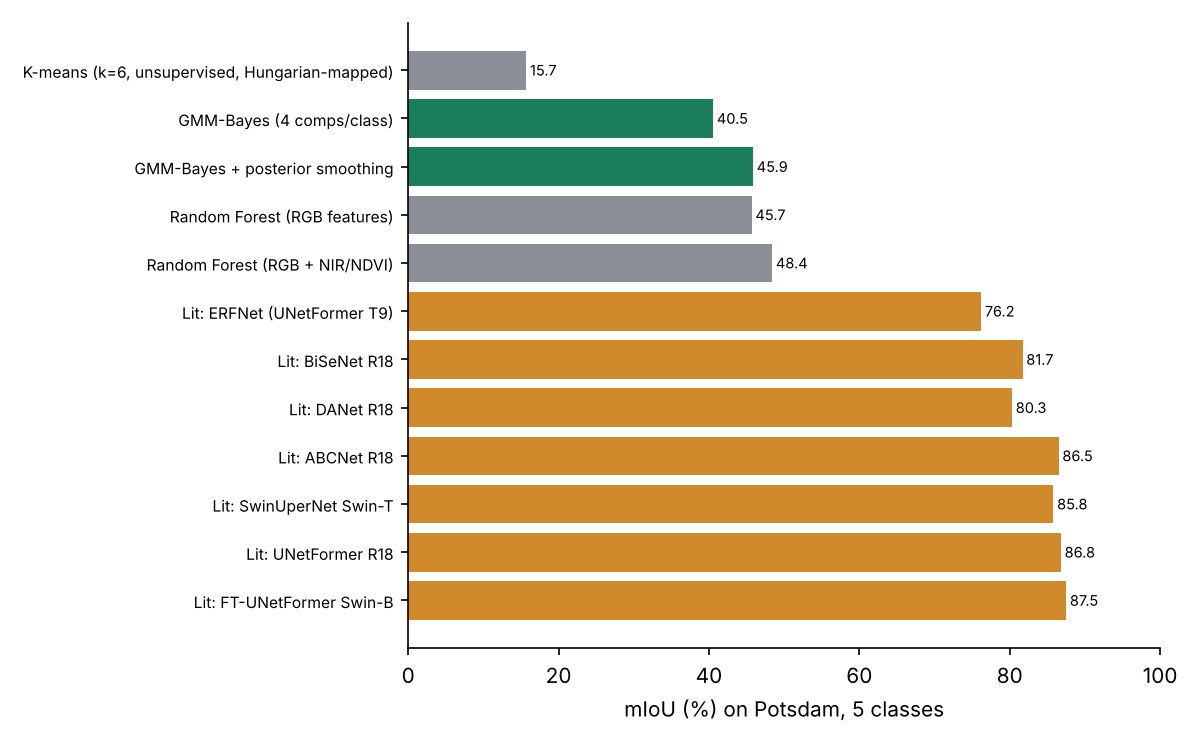
\includegraphics[width=.9\linewidth]{chart_potsdam.png}
\caption{Potsdam mIoU. Green/grey: classical pixel classifiers trained in minutes on CPU; orange: published deep models.}\end{figure}

\paragraph{Classical baselines -- what they teach.}
\begin{itemize}
\item \textbf{k-means (15.7 mIoU)}: colour clusters are not semantic classes (grey roofs = grey roads).
\item \textbf{GMM-Bayes (40.5)}: one 4-component GMM per class, Bayes rule with class priors -- a generative classifier.
\item \textbf{+ posterior smoothing (45.9)}: blurring the class posteriors (a cheap Markov-random-field/CRF surrogate)
adds 5.4 points: spatial context matters.
\item \textbf{Random forest (45.7) and RF + NIR/NDVI (48.4)}: the near-infrared band adds physics (chlorophyll
reflects NIR) and +2.7 points, mostly on impervious surfaces and buildings.
\item All are $\approx$40 points below deep models (86--88 mIoU): segmentation of buildings vs roads needs shape and
context that only a deep receptive field provides. \textbf{This is the honest argument for using a U-Net for
segmentation and GMMs only for triage/colour problems.}
\end{itemize}

\paragraph{Deep model (repo U-Net).} A time-boxed CPU training run of the repository's own model (filters=16) is
scheduled after this report; its numbers are added to Table~\ref{tab:potsdam} automatically by
\texttt{report/make\_assets.py}. Expected order of magnitude from the literature for a ResNet-18 U-Net baseline with GPU
training: 82.5 mIoU (UNetFormer ablation, Table 1 of Wang et al.\ 2022).

\section{Transfer to pathology segmentation}
Same code path for tumour segmentation on CAMELYON16: 256 tiles at 20$\times$, classes \{background, normal, tumour\}
(+ fluid/necrosis if annotated), Dice + CE loss, stain augmentation instead of colour jitter, overlap 50\% with
Gaussian-weighted blending, TTA, and a triage gate in front.
